\documentclass{standalone}
\usepackage{tikz}
\usepackage{ctex,siunitx}
\setCJKmainfont{Noto Serif CJK SC}
\usepackage{tkz-euclide}
\usepackage{amsmath}
\usepackage{wasysym}
\usetikzlibrary{patterns, calc}
\usetikzlibrary {decorations.pathmorphing, decorations.pathreplacing, decorations.shapes,}
\begin{document}
\small
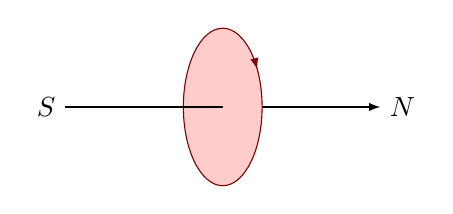
\begin{tikzpicture}[>=latex,scale=1]
  \draw[->](0,0)--(2,0)node[right]{$N$};
  \fill[red!20,draw=red!50!black,postaction={decorate},decoration={markings,mark=at position 0.1 with {\arrowreversed{>}}}](0,0)ellipse(0.5 and 1.0);
  \draw(-2,0)--(0,0)node[at start,left]{$S$};
\end{tikzpicture}
\end{document}